\chapter{METODOLOGIA}\label{cap:metodologia}

Para avaliação deste trabalho, foi considerada a base de dados
GrabCut~\cite{rother2004grabcut}, que contém 50 imagens com segmentação
binária e anotações parciais para execução de segmentações assistidas,
como a proposta de segmentação interativa.

As anotações parciais que serão consideradas neste trabalho são
chamadas de \textit{Lasso} e simulam um usuário realizando uma
marcação de regiões da imagem de fundo e primeiro plano para
segmentação. A anotação possui um esquema de anotação para treinamento
em escala de cinza e será descrita em sequência.

\begin{figure}[h!]
        \captionsetup{width=12cm}
		\Caption{\label{fig:grabcut-dataset}
          Exemplo de imagem dataset GrabCut com anotação parcial e
          a segmentação real (ground truth).
        }
		\centering
		\UFCfig{}{\fbox{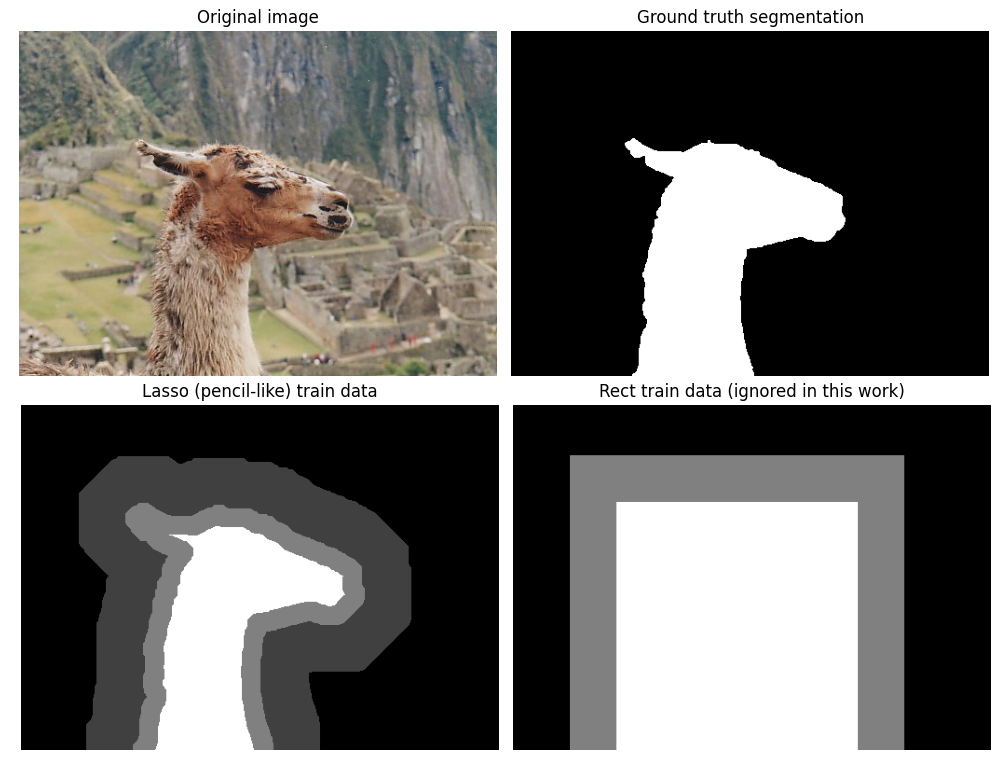
\includegraphics[width=12cm]{figuras/grabcut-dataset}}}{\Fonte{\fonteautor}}
\end{figure}
\FloatBarrier{}

\begin{table}[h]
  \centering
  \caption{Regras da anotação Lasso do GrabCut}
  \label{tab:grabcut-label}
  \begin{tabular}{lc}
    \toprule
    Descrição                                       & Nível de cinza \\
    \midrule \midrule
     fundo                                          & 0              \\
     fundo usado para \textbf{treinamento}          & 64             \\
     região de inferência                           & 128            \\
     primeiro plano usado para \textbf{treinamento} & 255            \\
    \bottomrule
  \end{tabular}
  \Fonte{\cite{rother2004grabcut}}
\end{table}


Através da Figura~\ref{fig:grabcut-dataset}, ao observar-se a primeira
imagem na segunda linha, tem-se a anotação \textit{Lasso}, na qual o
significado dos níveis de cinza pode ser visualizado na
Tabela~\ref{tab:grabcut-label}. Dessa maneira, para
treinamento\footnotemark{} são usados dois níveis de cinza: 64 para o
fundo e 255 para o primeiro plano.

\footnotetext{\gls{EGSIS} é um algoritmo transdutivo,
não existe treinamento, esses dados são apenas anotações parciais
que serão usadas para execução da inferência e obter a segmentação da
imagem.}

O método de avaliação consiste em executar o algoritmo desenvolvido
\gls{EGSIS} para essa base de dados e extrair métricas de qualidade de
segmentação para comparação com outros trabalhos, assim como estudo da
variação de parâmetros do modelo e a percepção de impacto nas métricas
de avaliação.

\section{Métricas de avaliação}\label{sec:metricas-avaliacao}

Para avaliação deste trabalho, foram selecionadas as seguintes métricas
que são comumente utilizadas para avaliação de segmentação de imagens:

\begin{enumerate}
\item \textit{Precision}
\item \textit{Recall}
\item \textit{F1 Score (Dice Coefficient)}
\item IoU
\end{enumerate}


\subsection{Precision}\label{sec:precision}

Para avaliação da precisão da segmentação, tem-se a seguinte definição:

\begin{equation}\label{eq:precision}
  Precision = \dfrac{TP}{TP + FP}
\end{equation}
\noindent
Em que \textit{TP} são os pixels classificados corretamente e \textit{FP}
os falsos-positivos. Essa métrica penaliza a presença de falsos
positivos. Quanto menos falsos-positivos, maior será a precisão.


\subsection{Recall}\label{sec:recall}

Para avaliação do \textit{Recall} (também conhecido como Sensibilidade), tem-se a seguinte definição:

\begin{equation}\label{eq:recall}
  Recall = \dfrac{TP}{TP + FN}
\end{equation}

Nessa equação, similar à precisão, é introduzido \textit{FN} no denominador,
os falsos-negativos. Diferentemente da precisão, o \textit{recall} penaliza
a presença de falso-negativos. Quanto menos falsos-negativos, maior
será o \textit{recall}.

\subsection{F1 Score}\label{sec:f1}

A métrica F1 Score, em segmentação de imagens também conhecida como
Dice Coefficient, é uma soma harmônica entre \textit{precision} e
\textit{recall}. Nessa situação, tem-se a definição:


\begin{equation}\label{eq:recall}
  F1 = \dfrac{2 \cdot Precision \cdot Recall}{Precision + Recall}
\end{equation}

F1 score é uma métrica balanceada que, entre \textit{precision} e \textit{recall},
penaliza a que tiver pior avaliação.

\subsection{IoU}\label{sec:iou}

IoU~\cite{rezatofighi2019generalized}, que significa
\textit{Intersection over Union}, é uma métrica popularmente usada
para medir a precisão de um objeto de segmentação em tarefas de visão
computacional, como detecção de objetos e segmentação semântica.

A métrica IoU calcula a proporção da área de interseção entre a região
estimada e a região real (ground truth) pela área da união dessas duas
regiões. A fórmula para calcular o IoU é:

\begin{equation}\label{eq:iou}
  IoU = \dfrac{\left| A \cap B \right|}{\left| A \cup B \right|}
\end{equation}


Nessa equação, $A$ e $B$ são matrizes de rótulos da imagem que serão
comparadas, sendo a matriz A os rótulos estimados e a matriz B os
reais. O valor de IoU varia de 0 a 1, com o valor 1 indicando uma
correspondência perfeita entre as regiões delimitadoras previstas e
reais, e o valor 0 indicando que não há sobreposição (pior valor). Em
geral, um IoU maior indica uma melhor precisão do modelo de
segmentação. Para ilustração, tem-se a seguinte figura~\ref{fig:iou}:

\begin{figure}[h!]
        \captionsetup{width=12cm}
		\Caption{\label{fig:iou}
          Ilustração das métricas IoU e F1 score.
        }
		\centering
		\UFCfig{}{\fbox{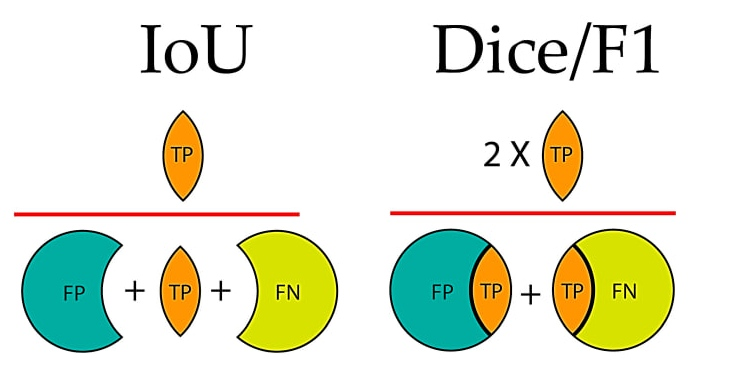
\includegraphics[width=12cm]{figuras/metrics}}}{\Fonte{\cite{maxwell2021metrics}}}
\end{figure}
\FloatBarrier{}
